
\section{Conclusion}

\subsection{Lessons learned}

The experience of applying the data model language, the model
catalogue, and the associated generation tools in the context of
clinical research informatics has led to the following suggestions.

\textsl{A data dictionary is not enough}. A simple, flat list of data
definitions does not support re-use at scale: it requires the user to
place all of the contextual information into the definition of each
data item, and mitigates against the automatic generation and
application of definitions.  Instead, we require a model catalogue, in
which every data element or class is defined in context.

\textsl{A catalogue is not enough}.  The models in the catalogue must
be linked to implementations, and to each other, with a considerable
degree of automatic support.  If the models are out of sync with the
implementations, and with the data, then their value is sharply
diminished.  Model-driven engineering is needed.

\textsl{The tools must be usable by domain experts}. To have the
processes of model creation and maintenance mediated by software
engineers is problematic: there may be misunderstandings regarding
interpretation, but---more importantly---there are not enough software
engineers to go around.  

\textsl{Many of the familiar} 

 this readability applies to the development interface, this is
  the interface that you want to use (can't do the turn time) - and
  you need to be able to pair program with domain experts
\textsl{A} you want inheritance within models, and include/import across
  models (start thinking of the models as code, although this is about
  managing information in general - managing declarations - it is
  coincidental that we are generating artefacts from them)
\textsl{B} you may want different types of model for different generated
  artefacts---depending upon what, exactly, is in the generator code
  as parameters and additional information---it may be the same set of
  data points overall, but you might well have a different refactoring
  in Fowler terms
\textsl{C} version and store the generation code (!)
\textsl{D} tag the generated artefacts with a link back to the model
  catalogue (XML schemas in HIC!)
\textsl{E} you will want more models than you think: for example, consider
  the model of a clinical test; now think about how it is dropped into
  a pathway; you need the pathway model to tell you what the dataset
  means; it has added further context to the data element definitions
  (you could flatten this, but that's bad)
\textsl{F} automate aspects of model management---versioning and dealing
  with multiple models
  \begin{itemize}
  \item automatically create (and propose) links, including
    classifications
  \item have links for new version of (sequential), refactoring of
    (parallel), derived from (data concepts across models), same as
    (strong assertion)
  \item use links in model maintenance - note that the definition that
    this was derived from has changed
  \item have publication cycle---a published model is for life
  \end{itemize}
\textsl{G} general lesson: if you want to manage data semantics, you need a
  compositional approach---none of this central coordination of a
  single data dictionary, none of this single hierarchy of data
  elements, none of this element by element description (all the
  context in the text of the element definition?  doesn't work!)
\textsl{H} general lesson: if you are going to manage data at scale, you
  need data model driven approach
\textsl{I} general lesson: if you have a model driven approach (data model
  or otherwise) then your management of models has all the same
  challenges as management of source code (you need an IDE) - really,
  if you are using models as programs, then you need to support them
  as programs

\clearpage

\begin{figure*}[h]
  \centering
  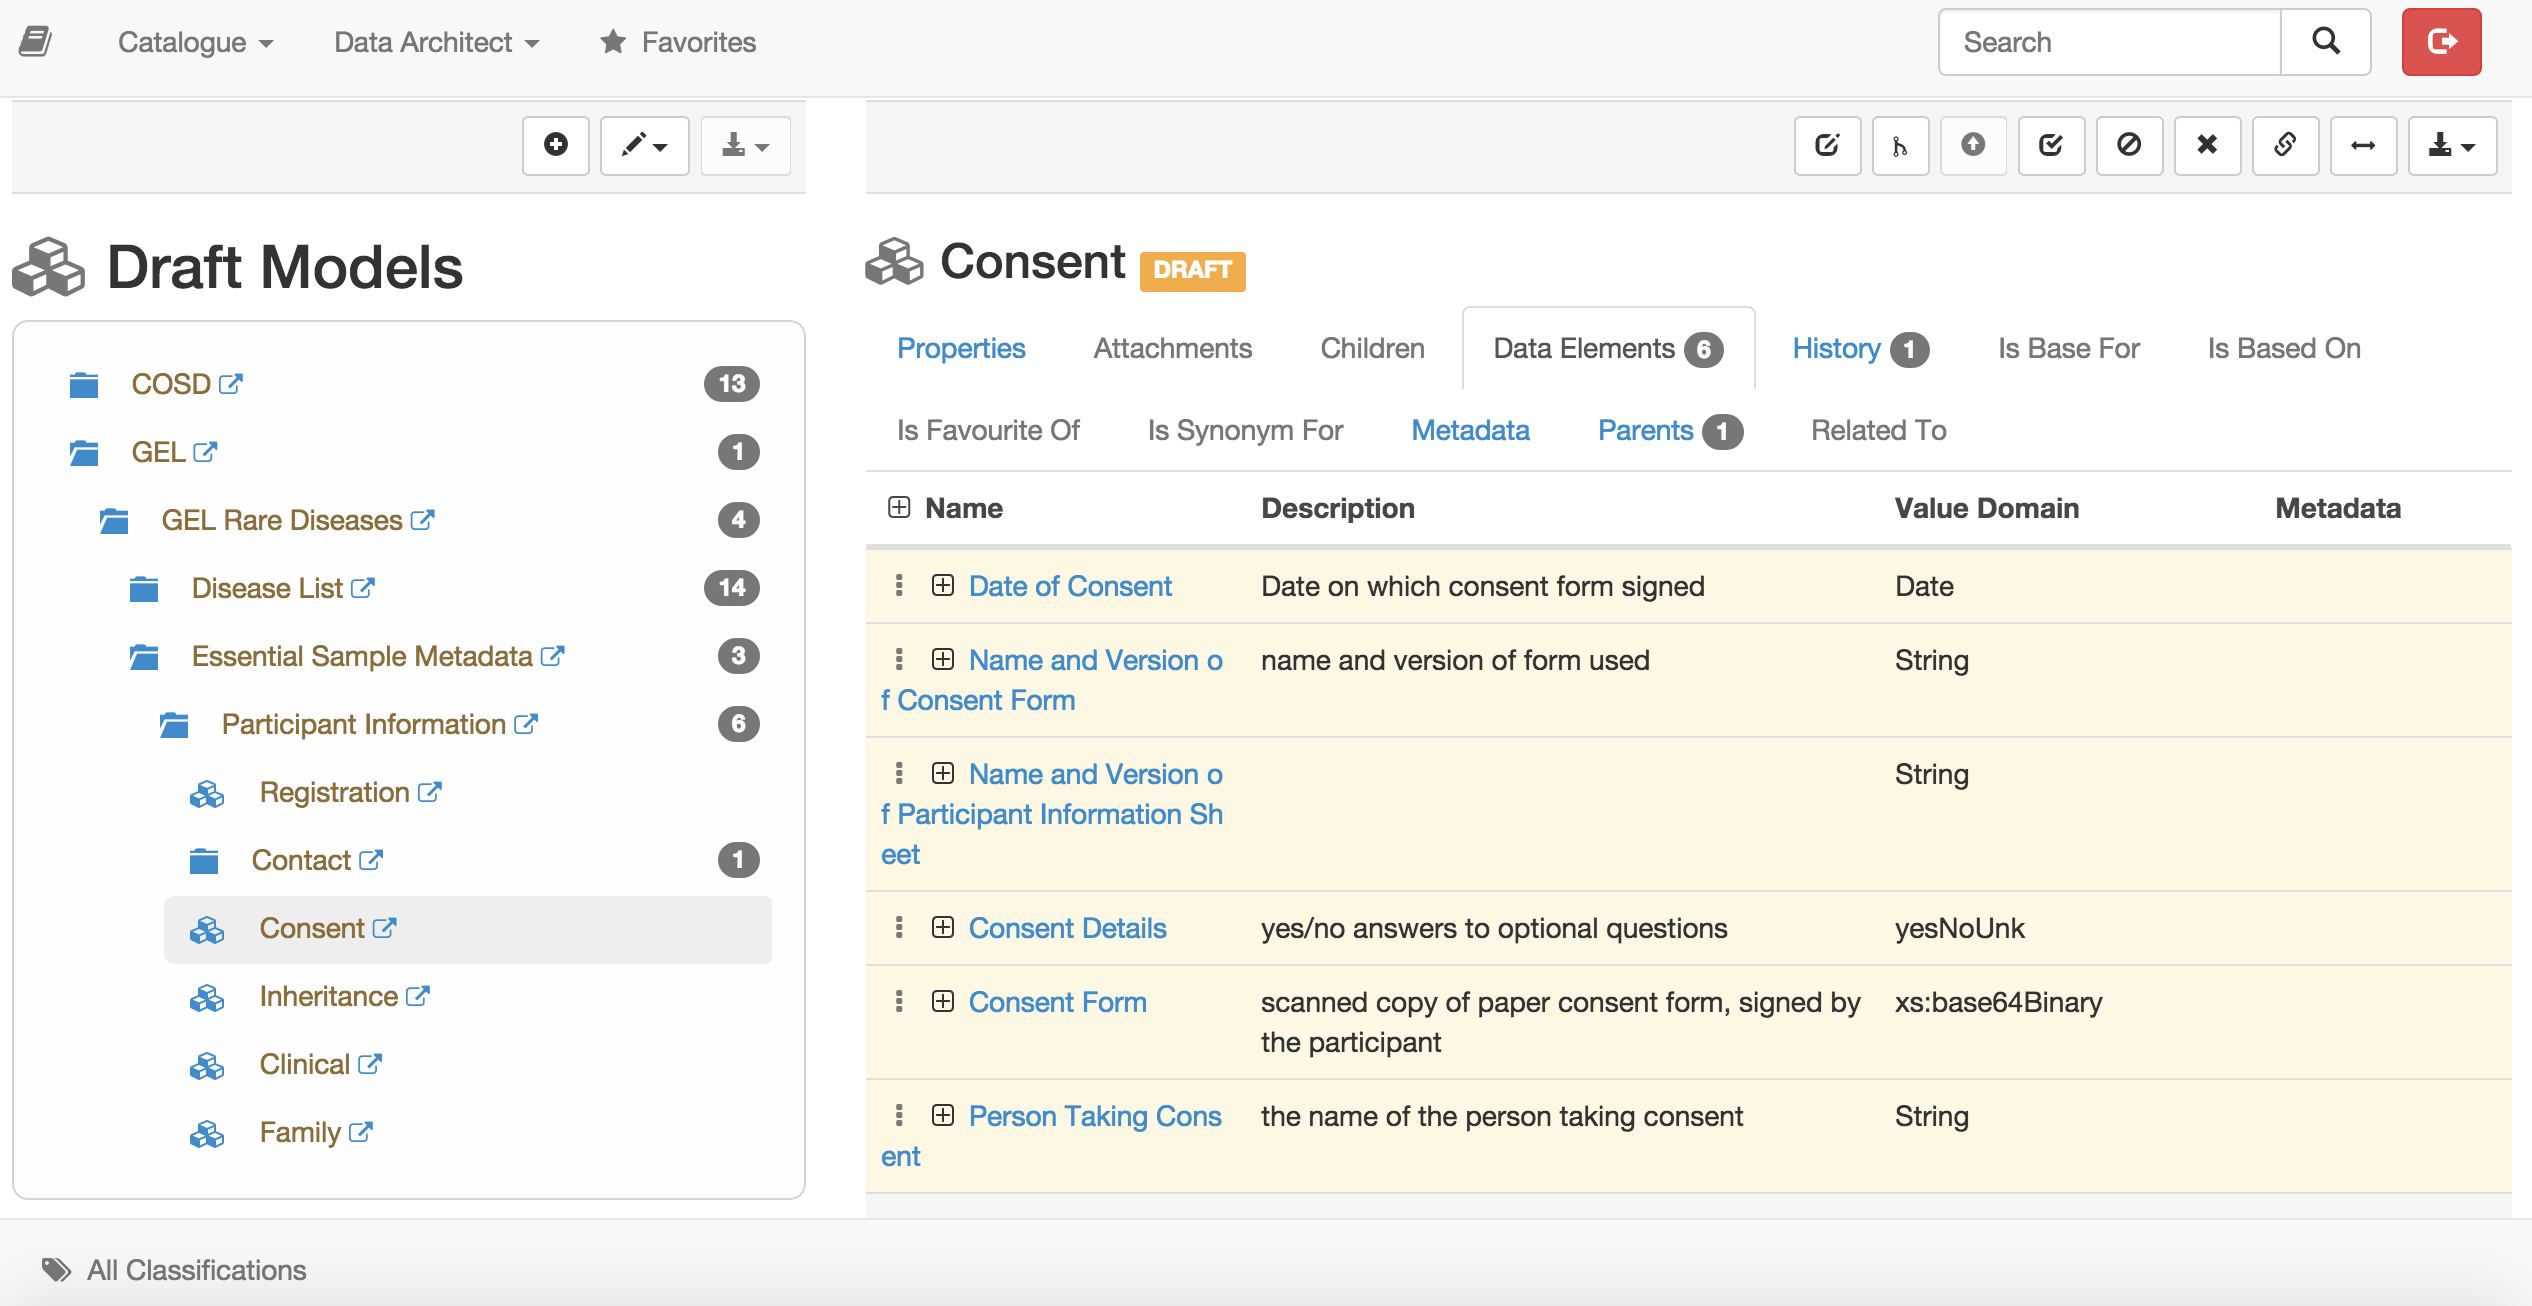
\includegraphics[width=\textwidth]{ScreenShot1}
  \caption{web interface to the model catalogue}
  \label{fig:webinterface}
\end{figure*}

\begin{figure*}[h]
  \centering
  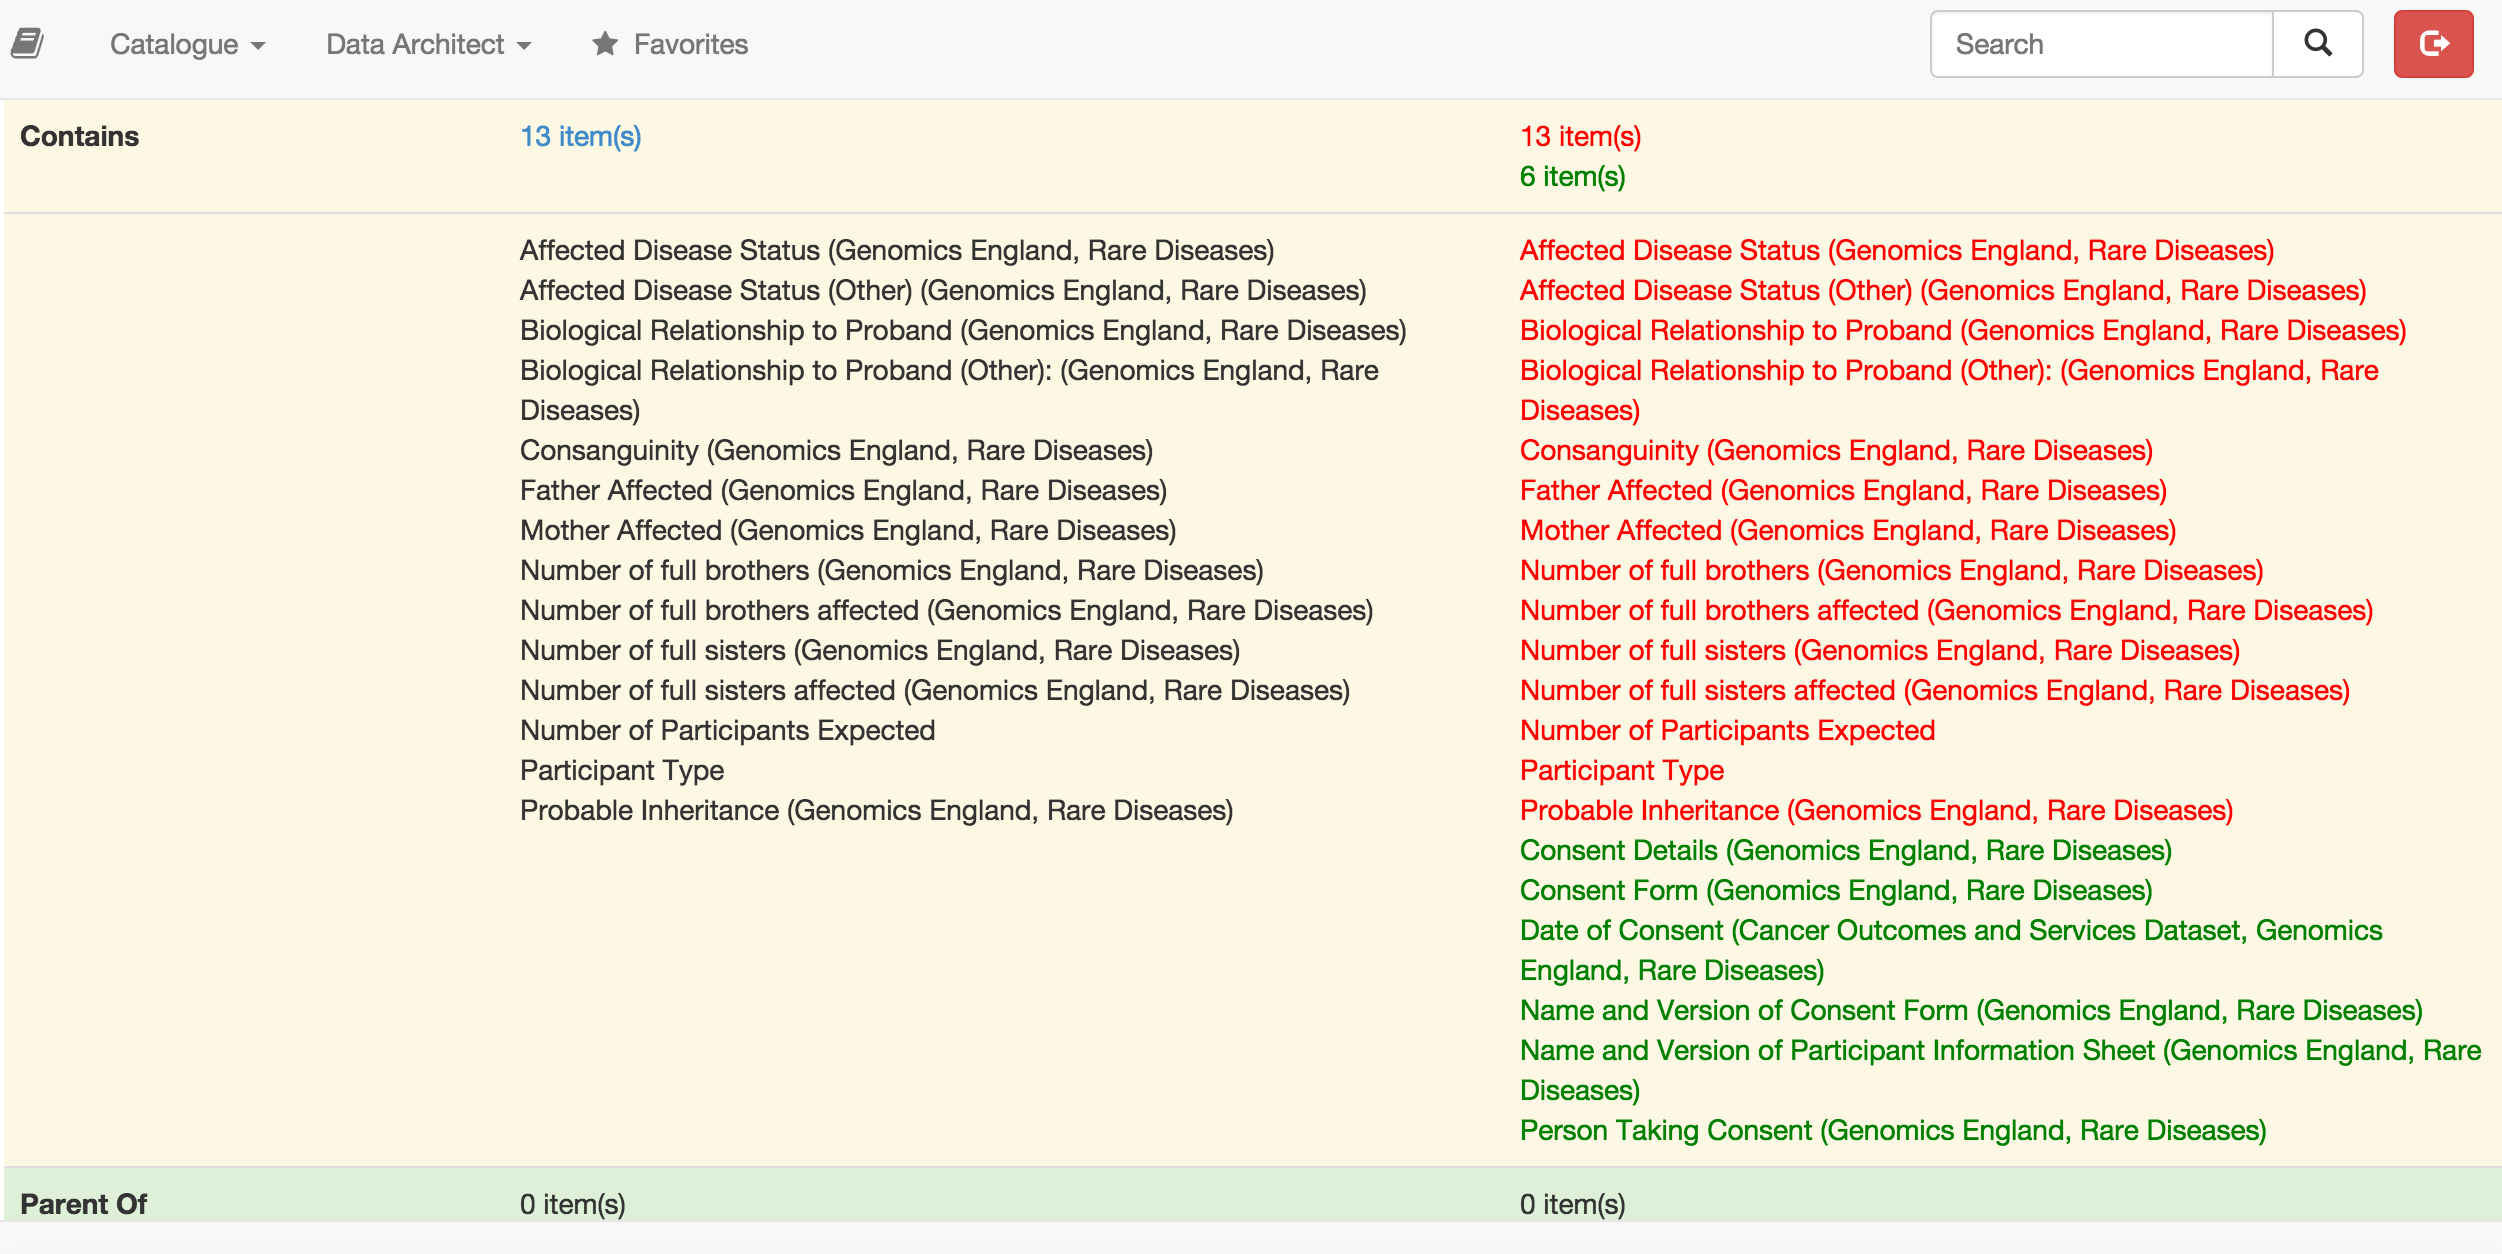
\includegraphics[width=\textwidth]{ScreenShot2}  
  \caption{automatic detection of model variation}
  \label{fig:variation}
\end{figure*}

